\clearpage
\chapter{EVALUACIÓN DE RESULTADOS}
\section{GENERACIÓN DE CASOS DE PRUEBA}
Para la elaboración de los casos de prueba se utilizo el siguiente programa en python para lograr general los números compuestos con las características que necesitamos.
\begin{lstlisting}[language=Python]
def primos_aleatorios_menores_a(n):
    primos = list(map(int, primos_list))
    upper = binary_search(n, primos)
    for i in range(6, 23):
        number = 1
        fact = []
        while math.log10(number) < i:
            x = random.randint(0, upper)
            prime = primos[x]
            number = number * prime
            fact.append(prime)
        print(f'{number} = {fact}')


def binary_search(x, array):
    a = 0
    b = len(array)
    while(b-a > 1):
        c = math.floor((b+a)/2)
        if array[c] > x:
            b = c
        else:
            a = c
    return a


def dos_primos_mitad_digitos():
    primos = list(map(int, primos_list))
    for i in range(6, 18):
        lower = binary_search(pow(10, i/2), primos)
        upper = binary_search(pow(10, (i/2)+1), primos)
        n1 = random.randint(lower, upper+1)
        n2 = random.randint(lower, upper + 1)
        number = primos[n1] * primos[n2]
        fact = [primos[n1], primos[n2]]
        print(f'{number} = {fact}')


def dos_primos_cercanos():
    primos = list(map(int, primos_list))
    for i in range(6, 18):
        lower = binary_search(pow(10, i/2), primos)
        upper = binary_search(pow(10, (i/2)+1), primos)
        n1 = random.randint(lower, upper+1)
        n2 = n1 + random.randint(0, 100)*(-1**random.randint(0, 10))
        number = primos[n1] * primos[n2]
        fact = [primos[n1], primos[n2]]
        print(f'{number} = {fact}')
\end{lstlisting}

\section{RECOLECCIÓN DE DATOS}
Para evaluar las propiedades de los algoritmos de factorización de números enteros, se intentara factorizar diferentes números, de diferentes tamaños, y que cumplen ciertas propiedades, utilizando los algoritmos de Divisiones Sucesivas, Algoritmo de Fermat,Algoritmo de Pollard Rho, Método de factorización por curva elíptica y Criba Cuadrática, Se variaron los parámetros de entrada de cada algoritmo para evaluarlos en cuanto a tiempo de ejecución, memoria utilizada y factores primos encontrados.

Tenemos 3 conjuntos te números, en la Tabla \ref{tabla:factores_pequeños} tenemos el primer conjunto de números los cuales tienen la particularidad de tener varios factores primos pequeños.

\begin{table}[H]
    \begin{adjustbox}{width=\columnwidth,center}
    \centering
    \begin{tabular}{|c|c|c|}
    \hline
    Número a Factorizar & Cantidad de Dígitos & Factores Primos \\
    \hline
    10856663 & 8 & [2267, 4789] \\
33391459 & 8 & [4327, 7717] \\
52863301961 & 11 & [2903, 3257, 5591] \\
60176508803 & 11 & [2399, 4931, 5087] \\
198506677433 & 12 & [2459, 8839, 9133] \\
212154123015013 & 15 & [2909, 3221, 4057, 5581] \\
224446720764659 & 15 & [1019, 3571, 6269, 9839] \\
178466784060619 & 15 & [577, 3527, 8933, 9817] \\
191470730623531 & 15 & [1373, 2347, 6361, 9341] \\
1422516521828333 & 16 & [3797, 4391, 9001, 9479] \\
1151160785730511661 & 19 & [7, 479, 1069, 5653, 6367, 8923] \\
188790832382174409613 & 21 & [97, 1949, 2243, 6571, 7057, 9601] \\
1020515758802666029 & 19 & [607, 2663, 7621, 8861, 9349] \\
1724030839771633601827 & 22 & [431, 2333, 3359, 6709, 8369, 9091] \\
5433376091934805169983 & 22 & [599, 4001, 5393, 6067, 7927, 8741] \\
1524997222903385596412591 & 25 & [887, 1877, 2767, 2969, 3049, 3889, 9403] \\
39926046905882865492053 & 23 & [643, 821, 1213, 1613, 2143, 2797, 6449] \\
    \hline
    \end{tabular}
\end{adjustbox}
    \caption{Casos de prueba: factores pequeños}
    \label{tabla:factores_pequeños}
    

\end{table}
    

En la Tabla \ref{tabla:factores_mitad} tenemos el siguiente conjunto de casos de prueba los cuales son el producto de dos números primos de aproximadamente la mitad de dígitos.

\begin{table}[H]
    \centering
    \begin{tabular}{|c|c|c|}
    \hline
    Número a Factorizar & Cantidad de Dígitos & Factores Primos \\
    \hline
    16236991 & 8 & [3361, 4831] \\
    469526207 & 9 & [18587, 25261] \\
    914465141 & 9 & [20731, 44111] \\
    45774604399 & 11 & [211193, 216743] \\
    138426627499 & 12 & [225343, 614293] \\
    2002311773621 & 13 & [703709, 2845369] \\
    36162913278367 & 14 & [4352419, 8308693] \\
    279747589361921 & 15 & [9353483, 29908387] \\
    3064287451898711 & 16 & [38873827, 78826493] \\
    6587155271801233 & 16 & [64776983, 101689751] \\
    853877380996470053 & 18 & [893082227, 956101639] \\
    831279571604286949 & 18 & [849122999, 978986051] \\
    37351160168752886641 & 20 & [5814185473, 6424143217] \\
    \hline
    \end{tabular}
    \caption{Casos de prueba: Dos primos de la mitad de dígitos}
    \label{tabla:factores_mitad}
    \end{table}
    

En la Tabla \ref{tabla:primos_cercanos} se encuentra el ultimo conjunto de casos de prueba los cuales son producto de dos números primos cercanos.

\begin{table}[H]
    \centering
    \begin{tabular}{|c|c|c|}
    \hline
    Número a Factorizar & Cantidad de Dígitos & Factores Primos \\
    \hline
66436879 & 8 & [8017, 8287] \\
686703811 & 9 & [25981, 26431] \\
8101438039 & 10 & [89963, 90053] \\
85526931211 & 11 & [292183, 292717] \\
262209534767 & 12 & [511991, 512137] \\
715281207649 & 12 & [845623, 845863] \\
1873966393597 & 13 & [1368467, 1369391] \\
18701749916023 & 14 & [4324261, 4324843] \\
1757788889012333 & 16 & [41925839, 41926147] \\
34843998810184129 & 17 & [186665113, 186665833] \\
874655409151893869 & 18 & [935229067, 935231207] \\
286073409635796583 & 18 & [534857399, 534859217] \\
    \hline
    \end{tabular}
    \caption{Casos de prueba: Dos primos cercanos}
    \label{tabla:primos_cercanos}
    \end{table}
    

% Para cada uno de los algoritmos mencionados se presentara el mismo conjunto de números a factorizar, estos tendrán diferentes características y tamaños, podemos ver estos números en la Tabla 4.1.

% \begin{table}[H]
%     \centering
%     \begin{tabular}{ccc}
%     \toprule
%     Número a factorizar & Cantidad de Dígitos & Factores primos\\
%     \midrule
%     189031 & 6 & 19 * 9949\\
%     162167 & 6 & 257 * 631 \\
%     129859 & 6 & 31 * 59 * 71\\
%     1456489 & 7 & 157 * 9277\\
%     4051247 & 7 & 1607 * 2521\\
%     1759875 & 7 & 3 * 5*5*5*13*19*19 \\
%     12345679 & 8 & 37 * 900361\\
%     47934097 & 8 & 5101 * 9397\\
%     61247841 & 8 & 3 * 59 * 293 * 1181\\
%     13290059 & 8 & 3119 * 4261\\
%     299944727 & 9 & 15013 * 19979\\
%     123456797 & 9 & 73 * 1691189\\
%     106418569 & 9 & 7901*13469\\
%     182552955 & 9 & 3*5 * 13 * 13*23*31*101\\
%     9872747167 & 10 & 71*9871*14087\\
%     1040594999 & 10 & 25453 * 40883\\
%     98765432101 & 11 & 7* 149* 94693607\\
%     98765432057 & 11 & 41 * 2408912977\\
%     29111611559 & 11 & 69763*417293\\
%     947452370929 & 12 & 597827*1584827\\
%     254903331620 & 12 & 2*2*5*7*137*13290059\\
%     5228595324973 & 13 & 7501367*697019\\
%     47096679270259 & 14 & 3986929*11812771\\
%     235308795456937 & 15 & 13895201*16934537\\
%     1536588216289253 & 16 & 27801481*55270013\\
%     71453335284995017 & 17 & 155267159*460196063\\
%     57639038785408205 & 17 & 5*107367629*107367629\\
%     123456789012345678 & 18 & 2*3*3*3*21491747*106377431\\
%     542588624267342771 & 18 & 999997717*542589863\\
%     75557863725914323419137 & 23 & 17 · 1217 · 148961 · 24517014940753\\
%     \bottomrule
%     \end{tabular}
%     \caption{Conjunto de casos de prueba}
%     \label{tab:test-cases}
% \end{table}

% Los anteriores números fueron escogidos bajo algún criterio, como ser que varios son producto de dos números primos de la mitad de digitos que el número a factorizar o que tengan factores primos cercanos entre si. Adicionalmente se probara con un conjunto aleatorio de números, los cuales se muestran en la siguiente tabla.

% \begin{table}[h!]
%     \centering
%     \begin{tabular}{ccc}
%     \toprule
%     Número a factorizar & Cantidad de Dígitos & Factores primos\\
%     \midrule
%     4301669863 & 10 & 19 * 9949\\
%     4474219569 & 10 & 19 * 9949\\
%     4664207327 & 10 & 19 * 9949\\
%     3058913425 & 10 & 19 * 9949\\
%     8483408929 & 10 & 19 * 9949\\
%     91157961540 & 11 & 19 * 9949\\
%     71834755526 & 11 & 19 * 9949\\
%     19273835063 & 11 & 19 * 9949\\
%     94619342089 & 11 & 19 * 9949\\
%     35787761525 & 11 & 19 * 9949\\
%     666487305812 & 12 & 19 * 9949\\
%     33597589296 & 11 & 19 * 9949\\
%     998954783887 & 12 & 19 * 9949\\
%     347170454804 & 12 & 19 * 9949\\
%     973310845497 & 12 & 19 * 9949\\
%     326766468166 & 12 & 19 * 9949\\
%     7801713685685 & 13 & 19 * 9949\\
%     2668814811683 & 13 & 19 * 9949\\
%     5166123625339 & 13 & 19 * 9949\\
%     1496809063452 & 13 & 19 * 9949\\
%     2381216947725 & 13 & 19 * 9949\\
%     9644598203024 & 13 & 19 * 9949\\
%     10767704951543 & 14 & 19 * 9949\\
%     39668435387513 & 14 & 19 * 9949\\
%     68567173978082 & 14 & 19 * 9949\\
%     626274576394575 & 15 & 19 * 9949\\
%     737718941804106 & 15 & 19 * 9949\\
%     801604699212680 & 15 & 19 * 9949\\
%     452737951177671 & 15 & 19 * 9949\\
%     651530963341522 & 15 & 19 * 9949\\
%     9042898512612678 & 16 & 19 * 9949\\
%     6834126780084647 & 16 & 19 * 9949\\
%     1975605261582842 & 16 & 19 * 9949\\
%     4052906513611024 & 16 & 19 * 9949\\
%     4218681717928292 & 16 & 19 * 9949\\
%     65120691164835513 & 17 & 19 * 9949\\
%     81771695091271478 & 17 & 19 * 9949\\
%     40037231406989079 & 17 & 19 * 9949\\
%     73220842553719932 & 17 & 19 * 9949\\
%     71476068120491844 & 17 & 19 * 9949\\
%     \bottomrule
%     \end{tabular}
%     \caption{Resultados del Modelo de Erdős-Rényi}
%     \label{tab:erdos-renyi}
% \end{table}

\section{RESULTADOS}
    \subsection{DIVISIONES SUCESIVAS}
    El algoritmo de divisiones sucesivas tiene una complejidad temporal de $O(\sqrt{n})$ en el peor caso y una complejidad espacial de $O(1)$. Se espera que este algoritmo se comporte bien cuando los factores primos son pequeños y en cuanto el factor más grande crezca este algoritmo dejara de ser adecuado. 

    Primero se realizara las pruebas con los casos de prueba de la Tabla \ref{tabla:factores_pequeños}
    
    \begin{table}[H]
        \centering
        \begin{adjustbox}{width=\columnwidth,center}
        \begin{tabular}{ccc}
        \toprule
        Número a factorizar & Tiempo de ejecución (ms) & Factores primos encontrados\\
        \midrule
        10856663 & 0.310 & [2267, 4789]\\
        33391459 & 0.464 & [4327, 7717]\\
        52863301961 & 0.386 & [2903, 3257, 5591]\\
        60176508803 & 0.339 & [2399, 4931, 5087]\\
        198506677433 & 0.555 & [2459, 8839, 9133]\\
        212154123015013 & 0.354 & [2909, 3221, 4057, 5581]\\
        224446720764659 & 0.570 & [1019, 3571, 6269, 9839]\\
        178466784060619 & 0.554 & [577, 3527, 8933, 9817]\\
        191470730623531 & 0.585 & [1373, 2347, 6361, 9341]\\
        1422516521828333 & 0.580 & [3797, 4391, 9001, 9479]\\
        1151160785730511661 & 0.545 & [7, 479, 1069, 5653, 6367, 8923]\\
        188790832382174409613 & 0.629 & [97, 1949, 2243, 6571, 7057, 9601]\\
        1020515758802666029 & 0.618 & [607, 2663, 7621, 8861, 9349]\\
        1724030839771633601827 & 0.652 & [431, 2333, 3359, 6709, 8369, 9091]\\
        5433376091934805169983 & 0.565 & [599, 4001, 5393, 6067, 7927, 8741]\\
        1524997222903385596412591 & 0.627 & [887, 1877, 2767, 2969, 3049, 3889, 9403]\\
        39926046905882865492053 & 0.434 & [643, 821, 1213, 1613, 2143, 2797, 6449]\\

        \bottomrule
        \end{tabular}
        \end{adjustbox}
    \caption{Resultados del Algoritmo de Divisiones Sucesivas para el conjunto de casos de prueba de la Tabla \ref{tabla:factores_pequeños}}
        \label{tab:res-trial_1}
    \end{table}

   Y ahora se realizara las pruebas con los casos de prueba de la Tabla \ref{tabla:factores_mitad}

    \begin{table}[H]
        \centering
        \begin{tabular}{ccc}
        \toprule
        Número a factorizar & Tiempo de ejecución (ms) & Factores primos encontrados\\
        \midrule
        16236991 & 0.295 & [3361, 4831]\\
        469526207 & 1.523 & [18587, 25261]\\
        914465141 & 2.715 & [20731, 44111]\\
        45774604399 & 14.768 & [211193, 216743]\\
        138426627499 & 37.848 & [225343, 614293]\\
        2002311773621 & 183.913 & [703709, 2845369]\\
        36162913278367 & 582.346 & [4352419, 8308693]\\
        279747589361921 & 2058.641 & [9353483, 29908387]\\
        3064287451898711 & 5634.140 & [38873827, 78826493]\\
        6587155271801233 & 7452.034 & [64776983, 101689751]\\
        853877380996470053 & 80050.156 & [893082227, 956101639]\\
        831279571604286949 & 76501.414 & [849122999, 978986051]\\
        37351160168752886641 & 768585.739 & [5814185473, 6424143217]\\

        \bottomrule
        \end{tabular}
        \caption{Resultados del Algoritmo de Divisiones Sucesivas para el conjunto de casos de prueba de la Tabla \ref{tabla:factores_mitad}}
        \label{tab:res-trial_2}
    \end{table}

    \begin{table}[H]
        \centering
        \begin{tabular}{ccc}
        \toprule
        Número a factorizar & Tiempo de ejecución (ms) & Factores primos encontrados\\
        \midrule
        66436879 & 0.437 & [8017, 8287]\\
        686703811 & 1.394 & [25981, 26431]\\
        8101438039 & 6.293 & [89963, 90053]\\
        85526931211 & 21.026 & [292183, 292717]\\
        262209534767 & 39.504 & [511991, 512137]\\
        715281207649 & 64.788 & [845623, 845863]\\
        1873966393597 & 109.328 & [1368467, 1369391]\\
        18701749916023 & 339.266 & [4324261, 4324843]\\
        1757788889012333 & 3414.500 & [41925839, 41926147]\\
        34843998810184129 & 15096.030 & [186665113, 186665833]\\
        874655409151893869 & 81195.058 & [935229067, 935231207]\\
        286073409635796583 & 43553.943 & [534857399, 534859217]\\

        \bottomrule
        \end{tabular}
        \caption{Resultados del Algoritmo de Divisiones Sucesivas para el conjunto de casos de prueba de la Tabla \ref{tabla:primos_cercanos}}
        \label{tab:res-trial-cercanos}
    \end{table}

    Como se puede ver este algoritmo funciona bastante bien cuando se tiene factores primos pequeños pero el tiempo de ejecución crece en gran medida cuando se tienen factores primos muy grandes y también se puede ver que este algoritmo devuelve todos los factores primos de los números a factorizar. Esto se puede notar mejor en el gráfico de la Figura \ref{fig:res-trial}
    

    \begin{figure}[H]
        \centering
        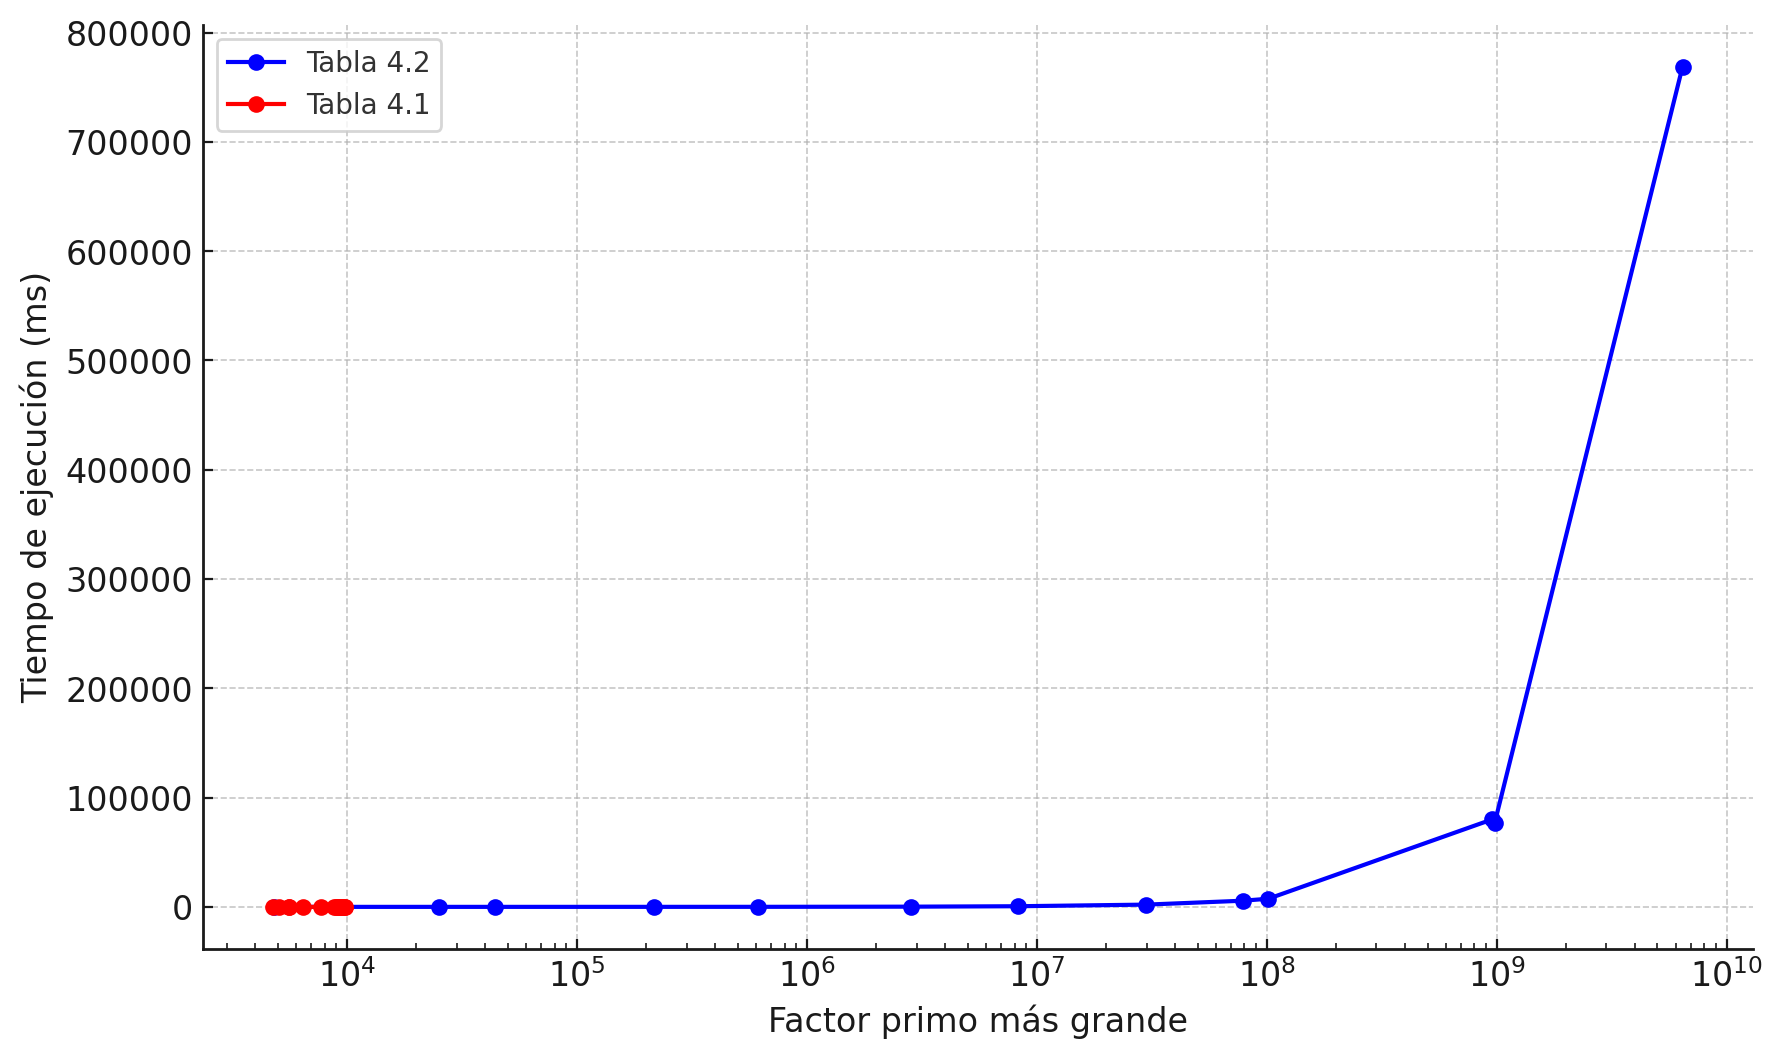
\includegraphics[width=\linewidth]{images/trial_divition3.png}
        \caption{Resultados Algoritmo de Divisiones Sucesivas}
        \label{fig:res-trial}
    \end{figure}

    \subsection{MÉTODO DE DIFERENCIA DE CUADRADOS DE FERMAT}
    El método de diferencia de cuadrados de Fermat tiene una complejidad temporal de $O(\sqrt{n})$ en el peor caso y una complejidad espacial de $O(1)$. Se espera que este algoritmo se desenvuelva bien cuando los factores primos sean cercanos y por la naturaleza de este algoritmo solo devolverá dos factores como resultado.

    Por este motivo primero se ejecutara el algoritmo con los casos de prueba de la Tabla \ref{tabla:factores_mitad}

    \begin{table}[H]
        \centering
        \begin{tabular}{ccc}
        \toprule
        Número a factorizar & Tiempo de ejecución (ms) & Factores primos encontrados\\
        \midrule
        16236991 & 0.026 & (3361, 4831)\\
        469526207 & 0.091 & (18587, 25261)\\
        914465141 & 0.602 & (20731, 44111)\\
        45774604399 & 0.007 & (211193, 216743)\\
        138426627499 & 13.287 & (225343, 614293)\\
        2002311773621 & 101.312 & (703709, 2845369)\\
        36162913278367 & 91.956 & (4352419, 8308693)\\
        279747589361921 & 879.645 & (9353483, 29908387)\\
        3064287451898711 & 1034.177 & (38873827, 78826493)\\
        6587155271801233 & 614.972 & (64776983, 101689751)\\
        853877380996470053 & 159.865 & (893082227, 956101639)\\
        831279571604286949 & 688.792 & (849122999, 978986051)\\
        37351160168752886641 & 2511.930 & (5814185473, 6424143217)\\
        \bottomrule
        \end{tabular}
        \caption{Resultados del Método de diferencia de cuadrados de Fermat con casos de prueba de la Tabla \ref{tabla:factores_mitad}}
        \label{tab:res-fermat-mitad}
    \end{table}

    Ahora se ejecutara el algoritmo con los casos de prueba de la Tabla \ref{tabla:primos_cercanos}, y se observara los resultados obtenidos:

    \begin{table}[H]
        \centering
        \begin{tabular}{ccc}
        \toprule
        Número a factorizar & Tiempo de ejecución (ms) & Factores primos encontrados\\
        \midrule
        66436879 & 0.009 & (8017, 8287)\\
        686703811 & 0.030 & (25981, 26431)\\
        8101438039 & 0.036 & (89963, 90053)\\
        85526931211 & 0.003 & (292183, 292717)\\
        262209534767 & 0.002 & (511991, 512137)\\
        715281207649 & 0.002 & (845623, 845863)\\
        1873966393597 & 0.002 & (1368467, 1369391)\\
        18701749916023 & 0.002 & (4324261, 4324843)\\
        1757788889012333 & 0.002 & (41925839, 41926147)\\
        34843998810184129 & 0.002 & (186665113, 186665833)\\
        874655409151893869 & 0.002 & (935229067, 935231207)\\
        286073409635796583 & 0.002 & (534857399, 534859217)\\
        \bottomrule
        \end{tabular}
        \caption{Resultados del Método de diferencia de cuadrados de Fermat con casos de prueba de la Tabla \ref{tabla:primos_cercanos}}
        \label{tab:res-fermat-cercano}
    \end{table}

    Se puede ver que este algoritmo funciona mejor cuando la distancia entre ambos factores es pequeña, lo cual puede ser visto de manera gráfica en la Figura \ref{fig:res-fermat}

    \begin{figure}[H]
        \centering
        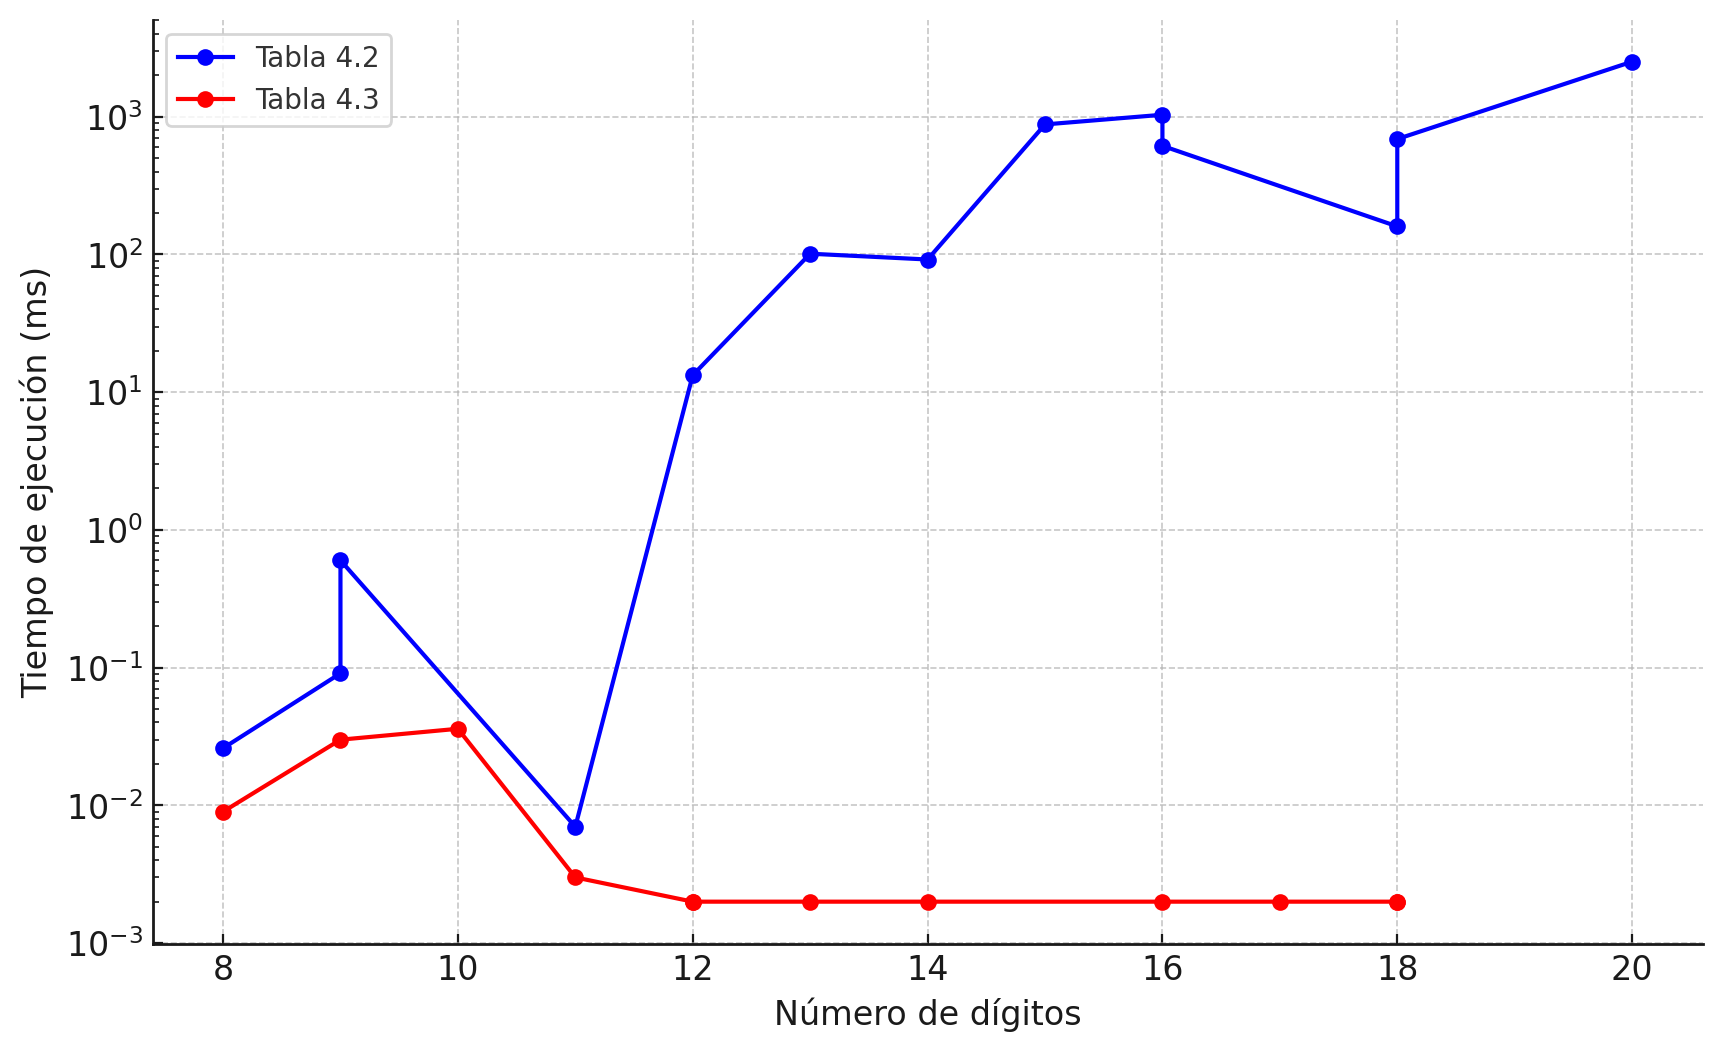
\includegraphics[width=\linewidth]{images/fermat_result.png}
        \caption{Resultados Método de diferencia de cuadrados de Fermat}
        \label{fig:res-fermat}
    \end{figure}

    \subsection{ALGORITMO DE POLLARD RHO}
    El algoritmo de Pollard Rho tiene una complejidad temporal de $O(n^{1/4})$ en el peor caso y una complejidad espacial de $O(1)$. Se espera que este algoritmo de uso general funcione bien para multiples casos.

    Comenzamos con los casos de prueba de la Tabla \ref{tabla:factores_pequeños}, que son números que tienen factores primos pequeños.

    \begin{table}[H]
        \centering
        \begin{adjustbox}{width=\columnwidth,center}
        \begin{tabular}{ccc}
        \toprule
        Número a factorizar & Tiempo de ejecución (ms) & Factores primos encontrados\\
        \midrule
        10856663 & 0.124 & [2267, 4789]\\
        33391459 & 0.035 & [4327, 7717]\\
        52863301961 & 0.219 & [2903, 3257, 5591]\\
        60176508803 & 0.181 & [2399, 4931, 5087]\\
        198506677433 & 0.242 & [2459, 9133, 8839]\\
        212154123015013 & 0.206 & [2909, 4057, 5581, 3221]\\
        224446720764659 & 0.324 & [1019, 9839, 3571, 6269]\\
        178466784060619 & 0.175 & [9817, 8933, 577, 3527]\\
        191470730623531 & 0.455 & [9341, 1373, 2347, 6361]\\
        1422516521828333 & 0.316 & [9479, 3797, 4391, 9001]\\
        1151160785730511661 & 0.656 & [7, 479, 1069, 8923, 5653, 6367]\\
        188790832382174409613 & 0.484 & [97, 7057, 6571, 1949, 2243, 9601]\\
        1020515758802666029 & 0.442 & [607, 7621, 2663, 8861, 9349]\\
        1724030839771633601827 & 0.481 & [431, 2333, 3359, 9091, 8369, 6709]\\
        5433376091934805169983 & 0.494 & [599, 4001, 8741, 7927, 5393, 6067]\\
        1524997222903385596412591 & 0.506 & [887, 2969, 3889, 1877, 2767, 3049, 9403]\\
        39926046905882865492053 & 0.316 & [1613, 995873, 643, 5993971, 6449]\\
        \bottomrule
        \end{tabular}
        \end{adjustbox}

        \caption{Resultados del Método de Pollard Rho con casos de la Tabla \ref{tabla:factores_pequeños}}
        \label{tab:res-pollard-rho-pequeños}
    \end{table}

    Ahora usaremos los casos de prueba de la Tabla \ref{tabla:factores_mitad}:

    \begin{table}[H]
        \centering
        \begin{tabular}{ccc}
        \toprule
        Número a factorizar & Tiempo de ejecución (ms) & Factores primos encontrados\\
        \midrule
        16236991 & 0.103 & [3361, 4831]\\
        469526207 & 0.215 & [25261, 18587]\\
        914465141 & 0.357 & [20731, 44111]\\
        45774604399 & 1.069 & [211193, 216743]\\
        138426627499 & 1.070 & [225343, 614293]\\
        2002311773621 & 1.553 & [703709, 2845369]\\
        36162913278367 & 4.246 & [4352419, 8308693]\\
        279747589361921 & 2.086 & [9353483, 29908387]\\
        3064287451898711 & 7.950 & [38873827, 78826493]\\
        6587155271801233 & 21.058 & [101689751, 64776983]\\
        853877380996470053 & 87.079 & [893082227, 956101639]\\
        831279571604286949 & 60.720 & [978986051, 849122999]\\
        37351160168752886641 & 64.655 & [6424143217, 5814185473]\\
        \bottomrule
        \end{tabular}
        \caption{Resultados del Método de Pollard Rho con casos de la Tabla \ref{tabla:factores_mitad}}
        \label{tab:res-pollard-rho-mitad}
    \end{table}

    Y por ultimo ejecutaremos el algoritmo con los casos de prueba de la Tabla \ref{tabla:primos_cercanos}
    
    \begin{table}[H]
        \centering
        \begin{tabular}{ccc}
        \toprule
        Número a factorizar & Tiempo de ejecución (ms) & Factores primos encontrados\\
        \midrule
        66436879 & 0.213 & [8287, 8017]\\
        686703811 & 0.235 & [25981, 26431]\\
        8101438039 & 0.280 & [90053, 89963]\\
        85526931211 & 2.490 & [292717, 292183]\\
        262209534767 & 1.729 & [511991, 512137]\\
        715281207649 & 1.384 & [845623, 845863]\\
        1873966393597 & 1.494 & [1369391, 1368467]\\
        18701749916023 & 0.481 & [4324843, 4324261]\\
        1757788889012333 & 15.424 & [41926147, 41925839]\\
        34843998810184129 & 14.593 & [186665113, 186665833]\\
        874655409151893869 & 62.654 & [935231207, 935229067]\\
        286073409635796583 & 11.130 & [534857399, 534859217]\\
        \bottomrule
        \end{tabular}
        \caption{Resultados del Método de Pollard Rho con casos de la Tabla \ref{tabla:primos_cercanos}}
        \label{tab:res-pollard-rho-cercanos}
    \end{table}

    En general para cualquier número Pollard-Rho tiene un tiempo de ejecución aceptable, con tiempos que no exceden los $100ms$ para nuestros casos de prueba, como se puede ver en la Figura \ref{fig:res-pollard-rho}.

    \begin{figure}[H]
        \centering
        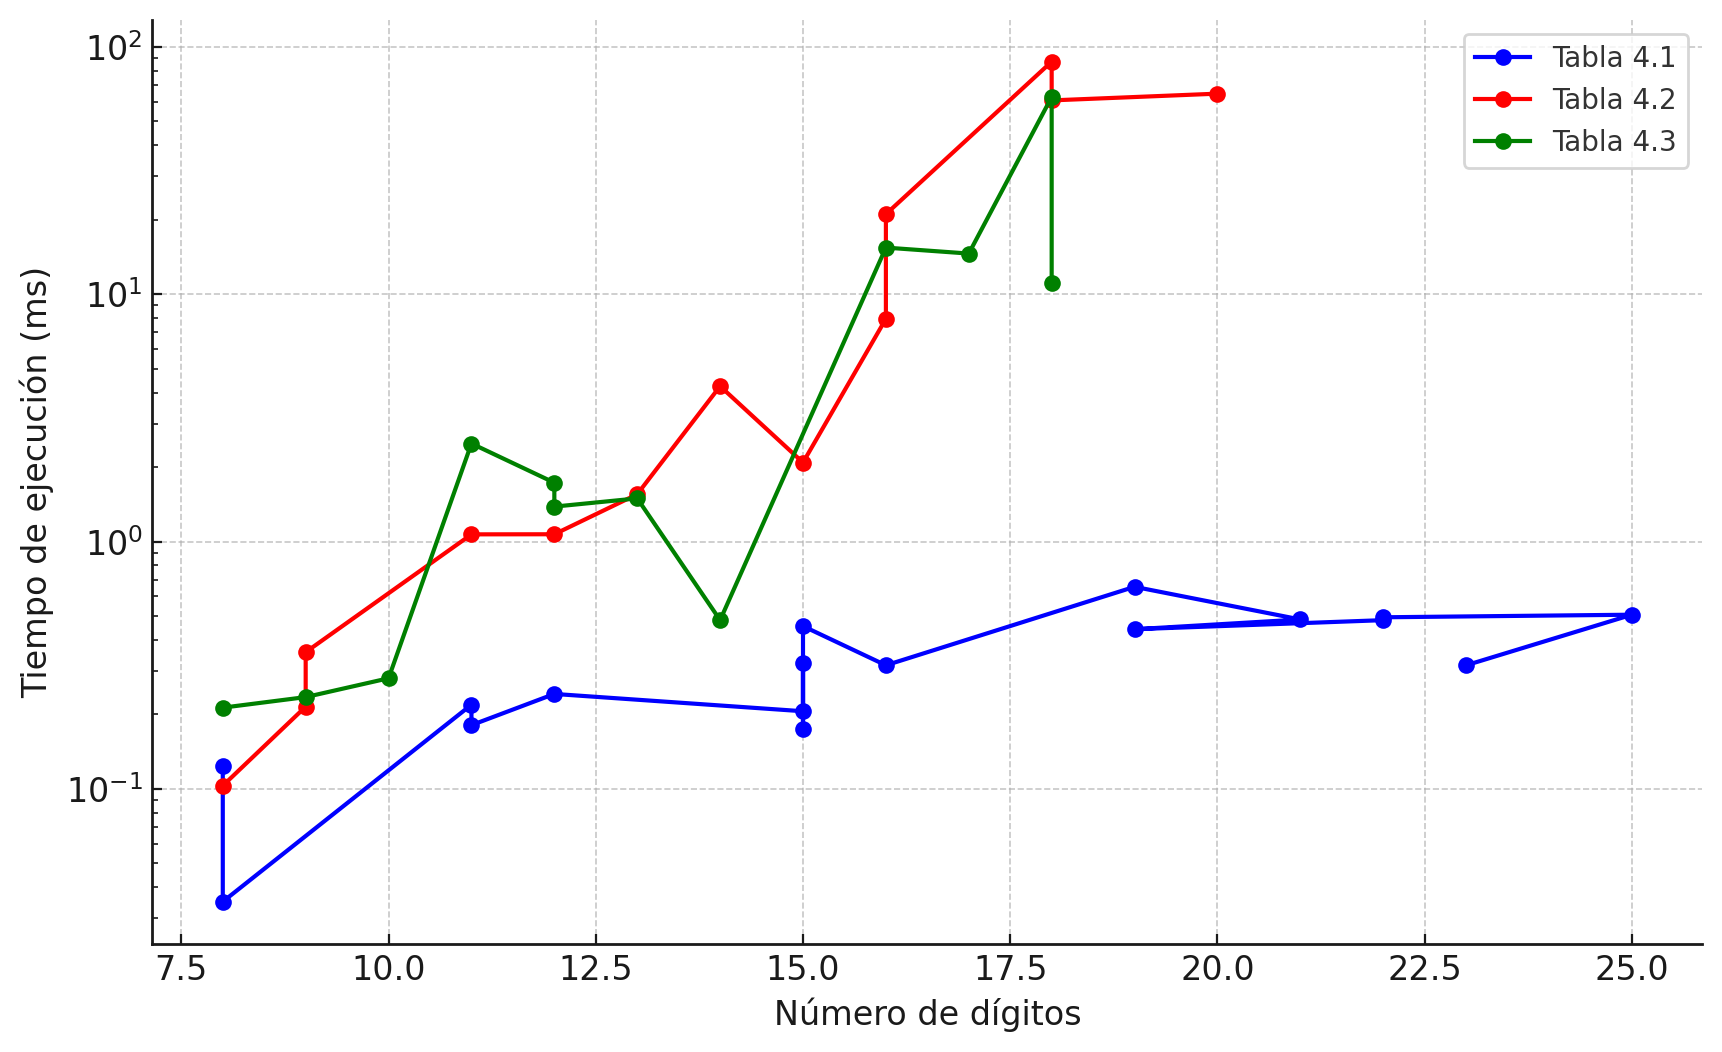
\includegraphics[width=\linewidth]{images/res-pollard-rho.png}
        \caption{Resultados Algoritmo de Pollard Rho}
        \label{fig:res-pollard-rho}
    \end{figure}

    \subsection{MÉTODO DE FACTORIZACIÓN CON CURVAS ELIPTICAS}
    El método de factorización con Curvas Elipticas tiene una complejidad temporal de \\ $O(e^{\sqrt{2 \log p \log \log p}})$ en el peor caso y una complejidad espacial de $O(\log n)$.

    \begin{table}[H]
        \centering
        \begin{tabular}{ccc}
        \toprule
        Número a factorizar & Tiempo de ejecución (ms) & Factores primos encontrados\\
        \midrule
        10856663 & 8.789 & 2267\\
        33391459 & 41.456 & 4327\\
        52863301961 & 15.100 & 2903\\
        60176508803 & 134.888 & 2399\\
        198506677433 & 274.809 & 2459\\
        212154123015013 & 28.153 & 2909\\
        224446720764659 & 224.039 & 1019\\
        178466784060619 & 2.281 & 577\\
        191470730623531 & 61.980 & 1373\\
        1422516521828333 & 67.354 & 4391\\
        1151160785730511661 & 0.041 & 7\\
        188790832382174409613 & 18.549 & 97\\
        1020515758802666029 & 1.148 & 607\\
        1724030839771633601827 & 9.571 & 3359\\
        5433376091934805169983 & 9.329 & 599\\
        1524997222903385596412591 & 22.790 & 2969\\
        39926046905882865492053 & 17.009 & 643\\

        \bottomrule
        \end{tabular}
        \caption{Resultados del Método de Factorización con Curvas Elipticas para los casos de prueba de la Tabla \ref{tabla:factores_pequeños}}
        \label{tab:res-eliptic-pequeños}
    \end{table}

    El método de curvas elípticas es rápido en general encontrando un primer factor, pero a medida que el numero crece se hace mas complicado hacer las cuentas geométricas para encontrar los factores primos.

    \begin{figure}[H]
        \centering
        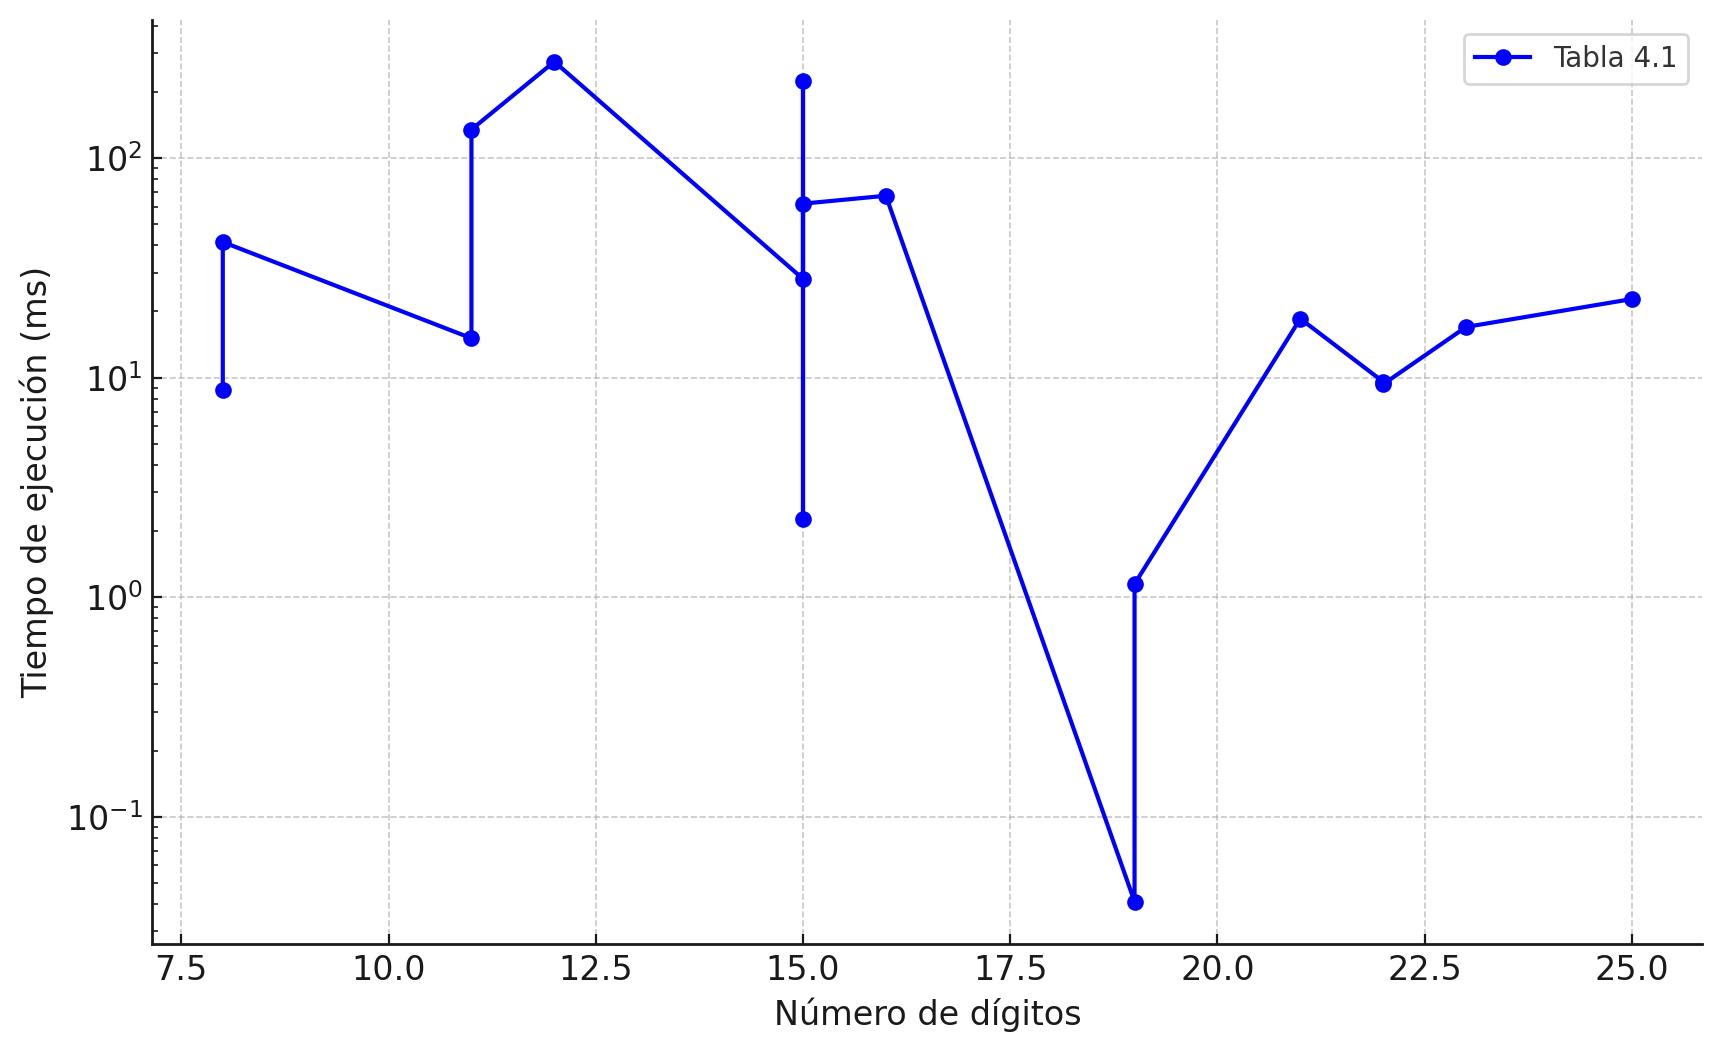
\includegraphics[width=\linewidth]{images/res-curva-eliptica.png}
        \caption{Resultados Método de Factorización con Curvas Elípticas con casos de prueba de la Tabla \ref{tabla:factores_pequeños}}
    \end{figure}

    \subsection{ALGORITMO DE FACTORIZACIÓN DE CRIBA CUADRÁTICA}
    El método de factorización de Criba Cuadrática tiene una complejidad temporal de \\ $O(e^{(1+o(n))\sqrt{\log n \log \log n}})$ en el peor caso.

    Para este algoritmo se usaran los casos de prueba de la Tabla \ref{tabla:factores_mitad} y Tabla \ref{tabla:primos_cercanos}
    \begin{table}[H]
        \centering
        \begin{tabular}{ccc}
        \toprule
        Número a factorizar & Tiempo de ejecución (ms) & Factores primos encontrados\\
        \midrule
        16236991 & 84.607 & [4831.0, 3361.0]\\
        469526207 & 51.509 & [25261.0, 18587.0]\\
        914465141 & 76.737 & [44111, 20731]\\
        45774604399 & 84.415 & [216743.0, 211193.0]\\
        138426627499 & 97.567 & [225343, 614293]\\
        2002311773621 & 92.401 & [703709, 2845369]\\
        36162913278367 & 99.894 & [4352419, 8308693]\\
        279747589361921 & 103.140 & [29908387, 9353483]\\
        3064287451898711 & 95.126 & [38873827, 78826493]\\
        6587155271801233 & 108.067 & [101689751, 64776983]\\

        \bottomrule
        \end{tabular}
        \caption{Resultados de la Factorización por Criba Cuadrática para los casos de prueba de la Tabla \ref{tabla:factores_mitad}}
        \label{tab:res-qs-mitad}
    \end{table}

    \begin{table}[H]
        \centering
        \begin{tabular}{ccc}
        \toprule
        Número a factorizar & Tiempo de ejecución (ms) & Factores primos encontrados\\
        \midrule
        66436879 & 69.424 & [8287.0, 8017.0]\\
        686703811 & 70.688 & [26431.0, 25981.0]\\
        8101438039 & 70.603 & [90053.0, 89963.0]\\
        85526931211 & 74.497 & [292717.0, 292183.0]\\
        262209534767 & 57.068 & [512137.0, 511991.0]\\
        715281207649 & 90.008 & [845863.0, 845623.0]\\
        1873966393597 & 82.297 & [1369391.0, 1368467.0]\\
        18701749916023 & 69.058 & [4324843.0, 4324261.0]\\
        1757788889012333 & 68.385 & [41926147.0, 41925839.0]\\
        \bottomrule
        \end{tabular}
        \caption{Resultados de la Factorización por Criba Cuadrática para los casos de prueba de la Tabla \ref{tabla:primos_cercanos}}
        \label{tab:res-qs-cercano}
    \end{table}

    \begin{figure}[H]
        \centering
        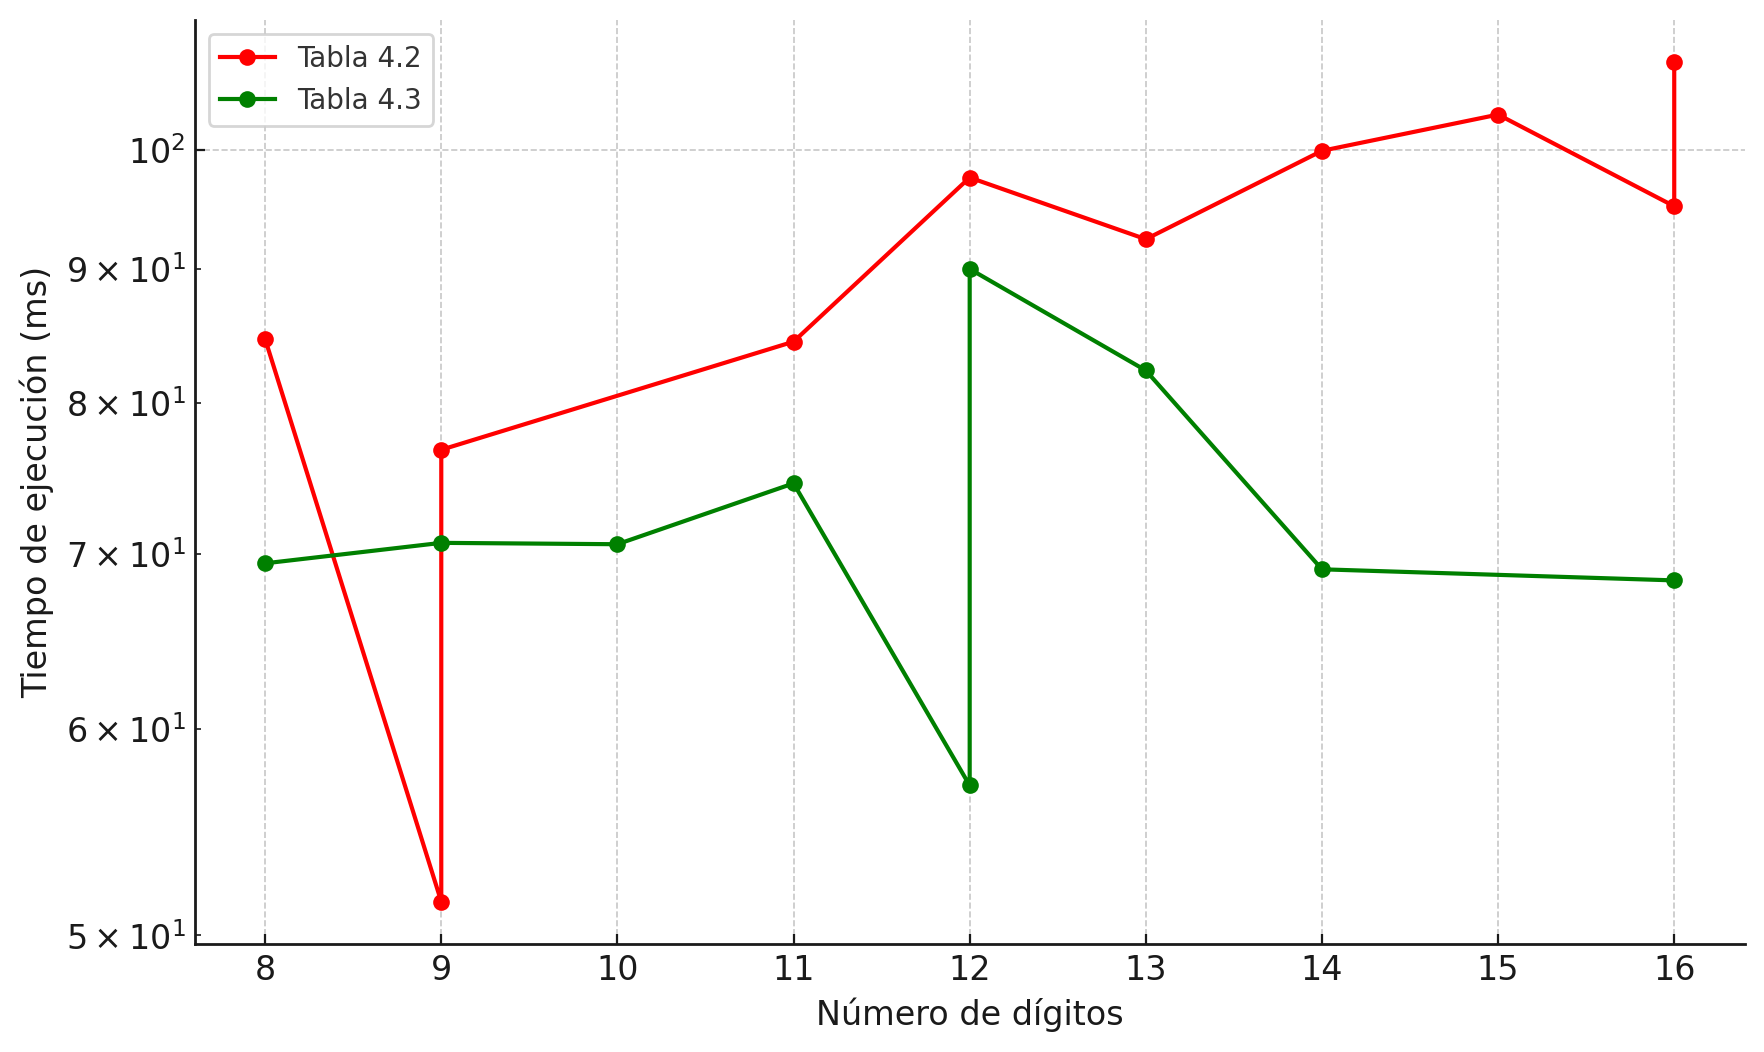
\includegraphics[width=\linewidth]{images/res-qs.png}
        \caption{Resultados la Factorización con Criba Cuadrática}
    \end{figure}

    % \subsection{MÉTODO DE FACTORIZACIÓN CON FRACCIONES CONTINUAS}
    % El método de factorización con Fracciones Continuas tiene una complejidad temporal de $O((\log n)^2)$ en el peor caso y una complejidad espacial de $O(\log n)$.

    \section{DEMOSTRACIÓN DE LA HIPÓTESIS}
    Para la demostración de la hipótesis se hará uso de los resultados obtenidos en las comparaciones, observando el tiempo de ejecución, el espacio de memoria utilizado y los factores primos encontrados.

    Para la prueba de hipotesis utilizaremos los resultados de los diferentes algoritmos con los casos de prueba de la Tabla \ref{tabla:primos_cercanos}.

    \begin{table}[H]
        \centering
        \begin{adjustbox}{width=\columnwidth,center}
        \begin{tabular}{|c|c|c|c|c|}
        \hline
        Número a factorizar & Divisiones Sucesivas & Fermat & Pollard Rho & Criba Cuadrática\\ \hline
        66436879        & 0.437                  & 0.009                  & 0.213                  & 69.424                 \\ \hline
        686703811       & 1.394                  & 0.03                   & 0.235                  & 70.688                 \\ \hline
        8101438039      & 6.293                  & 0.036                  & 0.28                   & 70.603                 \\ \hline
        85526931211     & 21.026                 & 0.003                  & 2.49                   & 74.497                 \\ \hline
        262209534767    & 39.504                 & 0.002                  & 1.729                  & 57.068                 \\ \hline
        715281207649    & 64.788                 & 0.002                  & 1.384                  & 90.008                 \\ \hline
        1873966393597   & 109.328                & 0.002                  & 1.494                  & 82.297                 \\ \hline
        18701749916023  & 339.266                & 0.002                  & 0.481                  & 69.058                 \\ \hline
        1757788889012333 & 3414.5                & 0.002                  & 15.424                 & 68.385                 \\ \hline
        34843998810184129 & 15096.03             & 0.002                  & 14.593                 &   103.500                     \\ \hline
        874655409151893869 & 81195.058           & 0.002                  & 62.654                 &  84.799                      \\ \hline
        286073409635796583 & 43553.943           & 0.002                  & 11.13                  &  88.860                      \\ \hline
        \end{tabular}
        \end{adjustbox}
        \caption{Tiempos de ejecución para diferentes algoritmos con los casos de prueba de la Tabla \ref{tabla:primos_cercanos}}
        \label{tabla:tiempos}
    \end{table}

    Comparación entre Divisiones Sucesivas y Algoritmo de Fermat:
    \[
        \text{Estadístico t: } 1.6454
    \]
    \[
        \text{Valor p: } 0.1281
    \]
    No se rechaza la hipótesis nula: no hay una diferencia significativa entre los algoritmos.


    Comparación entre Divisiones Sucesivas y Algoritmo Pollard-Rho
    \[
        \text{Estadístico t: } 1.6452
    \]
    \[
        \text{Valor p: } 0.1282
    \]
    No se rechaza la hipótesis nula: no hay una diferencia significativa entre los algoritmos.

    Comparación entre Divisiones Sucesivas y Criba Cuadratica
    \[
        \text{Estadístico t: } 1.6352
    \]
    \[
        \text{Valor p: } 0.1303
    \]
    No se rechaza la hipótesis nula: no hay una diferencia significativa entre los algoritmos.

    Comparación entre Algoritmo de Fermat y Algoritmo Pollard-Rho
    \[
        \text{Estadístico t: } -1.8211
    \]
    \[
        \text{Valor p: } 0.0959
    \]
    No se rechaza la hipótesis nula: no hay una diferencia significativa entre los algoritmos.

    Comparación entre Algoritmo de Fermat y Criba Cuadratica
    \[
        \text{Estadístico t: } -21.0917
    \]
    \[
        \text{Valor p: } 0.0000
    \]
    Rechazamos la hipótesis nula: hay una diferencia significativa entre los algoritmos.

    Comparación entre Algoritmo Pollard-Rho y Criba Cuadratica
    \[
        \text{Estadístico t: } -12.9675
    \]
    \[
        \text{Valor p: } 0.0000
    \]
    Rechazamos la hipótesis nula: hay una diferencia significativa entre los algoritmos.
